\documentclass[11pt]{article}
\usepackage{caption}
\usepackage{anysize}
\usepackage{fancyhdr}
\usepackage{graphicx}
\usepackage{subcaption}
\usepackage{color}
\usepackage{balance}
\usepackage{lipsum}
\usepackage{multirow}
\usepackage{multicol}
\usepackage{booktabs}
\usepackage{tikz}

\marginsize{.75in}{.75in}{.75in}{1in}
\pagestyle{fancy}
\rhead{\today}
\lhead{\includegraphics[height=2.0cm]{../logo.jpg}}
\rfoot{\thepage}
\cfoot{}
\renewcommand{\headrulewidth}{0pt} %removes line from fancy header
\renewcommand{\thispagestyle}[1]{} %placers header and footer on first page 
\renewcommand{\abstractname}{Summary}
\setlength{\columnsep}{25pt}
\date{}
\title{Laboratory Gasification Diagrams}

\begin{document}
\maketitle

%% %%%%%%%%%  %%
%% Furnace and Tube %%
%% %%%%%%%%%  %%

\begin{center}
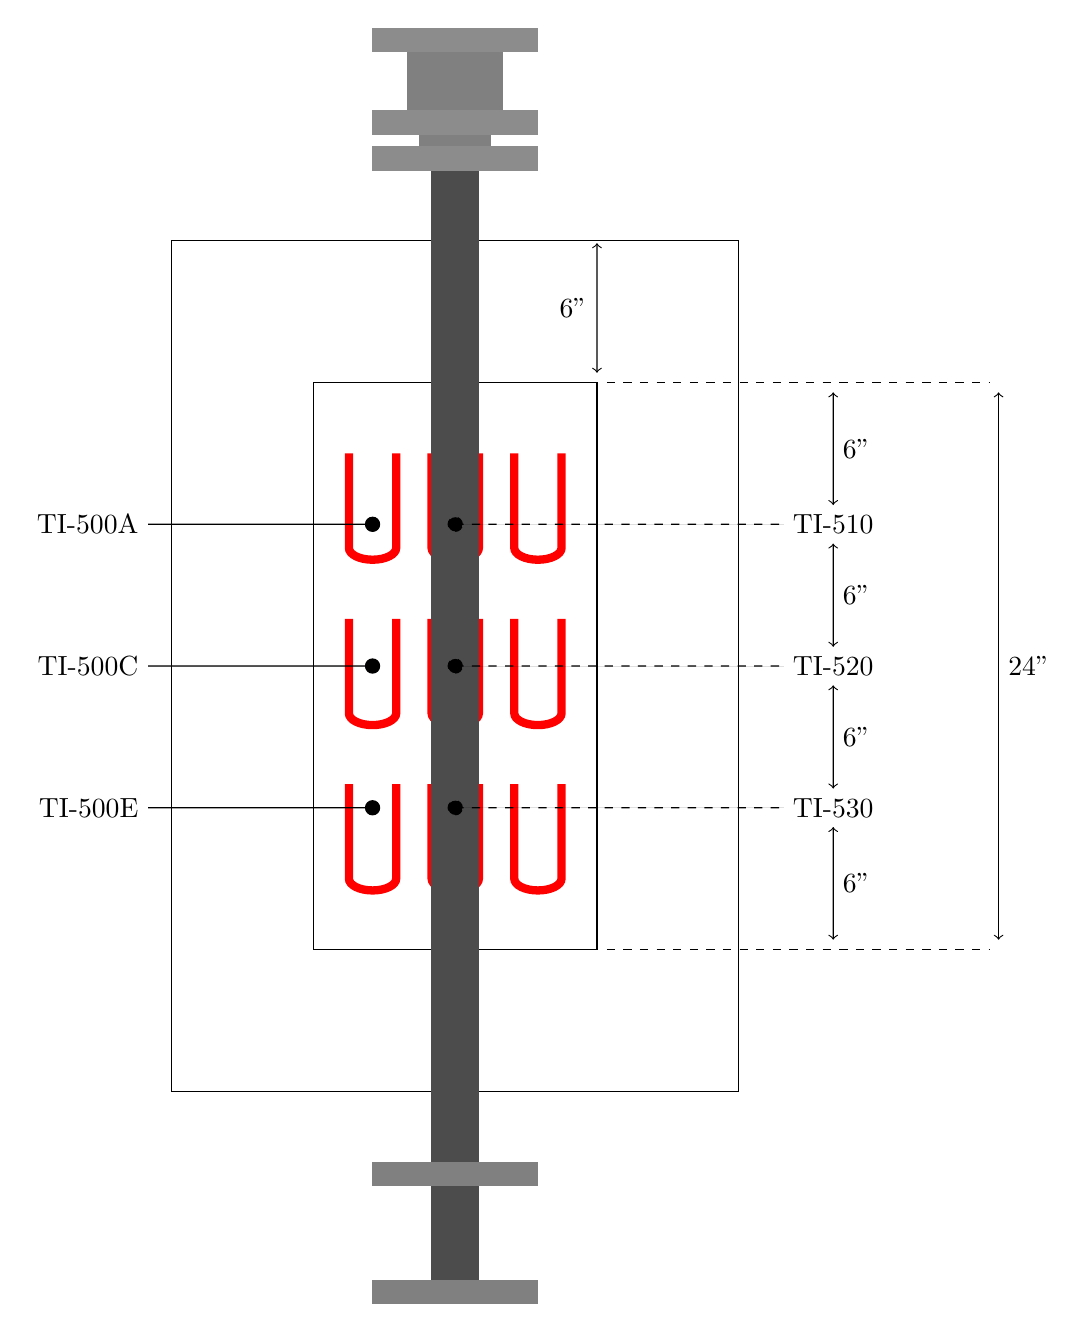
\begin{tikzpicture}[scale=0.3]
	\node (toprighthot) at (6,12) {};
	\node (bottomlefthot) at (-6,-12) {};
	\node (bottomrighthot) at (6,-12) {};
	\node (toplefthot) at (-6,12) {};
	\node (toprightbox) at (12,18) {};
	\node (topleftbox) at (-12,18) {};
	\node (bottomleftbox) at (-12,18) {};
	\node (bottomrightbox) at (12,-18) {};
	% Furnace Box %
	\draw (-12,-18) rectangle  (12,18);
	% Hot Zone %
	\filldraw [fill=red, fill opacity=0.0] (bottomlefthot) rectangle (toprighthot);
	% Elements %
	\foreach \y in {9, 2, -5}
		\foreach \x in {-4.5, -1, 2.5}
			{\draw [red,line width=3] (\x,\y) -- ++(0,-4) arc (180:360:1 and 0.5) -- ++(0,4);}
	% Tube %
	\filldraw [black!70!white] (-1,-27) rectangle (1,27);
	% Top Bucket %
	\filldraw [gray] (-1.5,21) rectangle (1.5,23.5);
	\filldraw [gray] (-2,23.5) rectangle (2,27);
	\filldraw [gray!90!white] (-3.5,21) rectangle (3.5,22);
	\filldraw [gray!90!white] (-3.5,22.5) rectangle (3.5,23.5);
	\filldraw [gray!90!white] (-3.5,26) rectangle (3.5,27);
	% Bottom Bucket %
	\filldraw [gray] (-3.5,-21) rectangle (3.5,-22);
	\filldraw [gray] (-3.5,-26) rectangle (3.5,-27);
	% Skin Thermocouples %
	\filldraw [black] (0,6) circle (0.3) [dashed] -- (16,6) node (ti510) [fill=white] {TI-510};
	\filldraw [black] (0,0) circle (0.3) [dashed] -- (16,0) node (ti520) [fill=white] {TI-520};
	\filldraw [black] (0,-6) circle (0.3) [dashed] -- (16,-6) node (ti530) [fill=white] {TI-530};
	\node (top510) at (16,12) {};
	\node (topright510) at (23,12) {};
	\node (bottom530) at (16,-12) {};
	\node (bottomright530) at (23,-12) {};
	\draw [<->] (top510) to node [auto] {6"} (ti510);
	\draw [<->] (ti510) to node [auto] {6"} (ti520);
	\draw [<->] (ti520) to node [auto] {6"} (ti530);
	\draw [<->] (ti530) to node [auto] {6"} (bottom530);
	\draw [<->] (topright510) to node [auto] {24"} (bottomright530);
	\draw [dashed] (toprighthot) -- (topright510);
	\draw [dashed] (bottomrighthot) -- (bottomright530);
	\draw [<->] (toprighthot) to node [auto] {6"} ++(0,5.9);
	
	% Element Thermocouples %
	\filldraw [black] (-3.5,6) circle (0.3) -- (-13,6) node (ti510) [anchor=east] {TI-500A};
	\filldraw [black] (-3.5,0) circle (0.3) -- (-13,0) node (ti520) [anchor=east] {TI-500C};
	\filldraw [black] (-3.5,-6) circle (0.3) -- (-13,-6) node (ti530) [anchor=east] {TI-500E};

\end{tikzpicture}
\end{center}

%% %%% %%
%% Lance %%
%% %%% %%	
	
\begin{center}
\begin{tikzpicture}

\end{tikzpicture}
\end{center}


%% %%%%%%%  %%
%% Flow Diagram %%
%% %%%%%%%  %%

\end{document}

